\documentclass{article}
\usepackage[utf8]{inputenc}
\usepackage[italian]{babel}
\usepackage{natbib}
\usepackage{graphicx}
\usepackage[table,xcdraw]{xcolor}
\usepackage{listings}
\usepackage{amsmath}
\usepackage{minted}
\usepackage{amsthm}
\usepackage{enumitem}
\usepackage{color}
\usepackage{svg}
\usepackage{pgfplots}
\usepackage[hidelinks]{hyperref}
\usepackage{xcolor,soul}
\definecolor{lightcyan}{rgb}{0.8,1,1}
\sethlcolor{lightcyan}

% ----- NEW SYMBOLS

\newcommand{\imgtick}{\ensuremath{%
  \mathchoice{
\includegraphics[height=2ex]{images/symbols/tick.png}}
    {
\includegraphics[height=2ex]{images/symbols/tick.png}}
    {
\includegraphics[height=1.5ex]{images/symbols/tick.png}}
    {
\includegraphics[height=1ex]{images/symbols/tick.png}}
}}

\newcommand{\imgminus}{\ensuremath{%
  \mathchoice{
\includegraphics[height=2ex]{images/symbols/minus.png}}
    {
\includegraphics[height=2ex]{images/symbols/minus.png}}
    {
\includegraphics[height=1.5ex]{images/symbols/minus.png}}
    {
\includegraphics[height=1ex]{images/symbols/minus.png}}
}}

\newcommand{\imgplus}{\ensuremath{%
  \mathchoice{
\includegraphics[height=2ex]{images/symbols/plus.png}}
    {
\includegraphics[height=2ex]{images/symbols/plus.png}}
    {
\includegraphics[height=1.5ex]{images/symbols/plus.png}}
    {
\includegraphics[height=1ex]{images/symbols/plus.png}}
}}

\newcommand{\imgx}{\ensuremath{%
  \mathchoice{
\includegraphics[height=2ex]{images/symbols/x.png}}
    {
\includegraphics[height=2ex]{images/symbols/x.png}}
    {
\includegraphics[height=1.5ex]{images/symbols/x.png}}
    {
\includegraphics[height=1ex]{images/symbols/x.png}}
}}

\newcommand{\imgdivided}{\ensuremath{%
  \mathchoice{
\includegraphics[height=2ex]{images/symbols/divided.png}}
    {
\includegraphics[height=2ex]{images/symbols/divided.png}}
    {
\includegraphics[height=1.5ex]{images/symbols/divided.png}}
    {
\includegraphics[height=1ex]{images/symbols/divided.png}}
}}

\newcommand{\imgchina}{\ensuremath{%
  \mathchoice{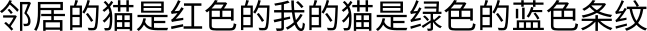
\includegraphics[height=2ex]{images/cinese_esempio.png}}
    {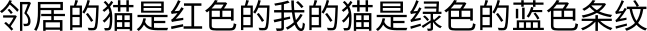
\includegraphics[height=2ex]{images/cinese_esempio.png}}
    {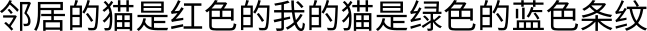
\includegraphics[height=1.5ex]{images/cinese_esempio.png}}
    {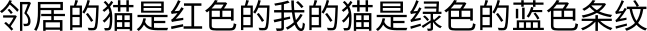
\includegraphics[height=1ex]{images/cinese_esempio.png}}
}}

\newcommand{\imgchinasplitted}{\ensuremath{%
  \mathchoice{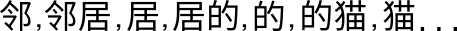
\includegraphics[height=2ex]{images/cinese_esempio_splitted.png}}
    {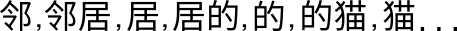
\includegraphics[height=2ex]{images/cinese_esempio_splitted.png}}
    {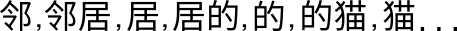
\includegraphics[height=1.5ex]{images/cinese_esempio_splitted.png}}
    {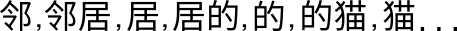
\includegraphics[height=1ex]{images/cinese_esempio_splitted.png}}
}}
\newcommand{\commonCrawlFilesTable}[0]{
    \renewcommand\arraystretch{1.2}
    % Please add the following required packages to your document preamble:
    % \usepackage{graphicx}
    % \usepackage[table,xcdraw]{xcolor}
    % If you use beamer only pass "xcolor=table" option, i.e. \documentclass[xcolor=table]{beamer}
    \begin{table}[h]
    \resizebox{\textwidth}{!}{%
    \begin{tabular}{lllr}
    \rowcolor[HTML]{C0C0C0} 
    Tipo File                                                          & Descrizione                                                                                                                                              & \#Files & \begin{tabular}[c]{@{}r@{}}Dim.dei file\\ compressi\end{tabular} \\ \hline
    \rowcolor[HTML]{EFEFEF} 
    Segments                                                           &                                                                                                                                                          & 100     &                                                                   \\
    WARC files                                                         & Dati grezzi generati dal Crawler                                                                                                                         & 64000   & 59.86 TiB                                                         \\
    \rowcolor[HTML]{EFEFEF} 
    WAT files                                                          & \begin{tabular}[c]{@{}l@{}}Contengono meta-dati relativi ai record nei \\ file WARC\end{tabular}                                                          & 64000   & 18.23 TiB                                                         \\
    WET files                                                          & \begin{tabular}[c]{@{}l@{}}Contengono solo testo semplice estratto \\ dai WARC\end{tabular}                                                              & 64000   & 7.62 TiB                                                          \\
    \rowcolor[HTML]{EFEFEF} 
    Robots.txt files                                                   & \begin{tabular}[c]{@{}l@{}}Files Robot.txt richiesti ai vari siti analizzati \\ (consentono al Crawler di scansionare \\ meglio i siti web)\end{tabular} & 64000   & 170 GiB                                                          \\
    \begin{tabular}[c]{@{}l@{}}Non-200 \\ responses files\end{tabular} & \begin{tabular}[c]{@{}l@{}}Risposte del server con HTTP status code \\ diverso da 200 (404, redirects, ecc.)\end{tabular}                                & 64000   & 1.79 TiB                                                          \\
    \rowcolor[HTML]{EFEFEF} 
    URL index files                                                    & \begin{tabular}[c]{@{}l@{}}Indice degli url analizzati, completo di utili \\ informazioni aggiuntive\end{tabular}                                        & 302     & 210 GiB                                                         
    \end{tabular}%
    }
    \end{table}
    \renewcommand\arraystretch{1.0}
}

%TOTALE: 88791
%tick: 49668
%x: 5371
%plus: 14058
%minus: 14941
%divided: 4753
\newcommand{\printHistogram}[0]{
    %\pgfplotsset{scaled y ticks=false}
    \begin{tikzpicture}
    \begin{axis}[
        symbolic x coords={\imgtick{},\imgx{},\imgplus{},\imgminus{},\imgdivided{}}, 
        ylabel = {occorrenze ($\cdot 10^3$)}, 
        xlabel = {Accuratezza dei risultati}, 
        xtick=data]
        
        \addplot[ybar,fill=white] coordinates {
            (\imgtick{}, 49.668)
            (\imgx{}, 5.371)
            (\imgplus{}, 14.058)
            (\imgminus{}, 14.941)
            (\imgdivided{}, 4.753)
        };
    \end{axis}
    \end{tikzpicture}
}

\newcommand{\printTimeGraph}[0]{
    \begin{tikzpicture}
    \begin{axis}[
      %ymin=20,
      %ymax=90,
      %width=15cm,
      %height=7cm,
      ylabel={tempo (minuti)},
      xlabel={\#files WET analizzati},
      %xticklabels={,2,4,6,8,10}, 
      legend style={at={(0.13,0.83)},
      anchor=west, legend columns=-1, font=\small},
      legend cell align=left,
      xtick=data
     ]

    \addlegendentry{abc}

    \addplot[blue, mark=+] coordinates {
        (2, 1.23)
        (4, 2.32)
        (6, 3.23)
        (8, 4.32)
        (10, 5.45)
    };
    
    \addplot[gray, mark=] coordinates {
        (2, 1.23)
        (4, 2.46)
        (6, 3.69)
        (8, 4.92)
        (10, 6.15)
    };
    \end{axis}
    \end{tikzpicture}
}

\setlist[itemize,1]{label=$\--$}

% ------------------- COMMANDS
\newcommand{\MR}{MapReduce}
%\newcommand{\MRA}{MR Lang Analyzer}
\newcommand{\cld}{\textit{CLD}2}
\newcommand{\WET}{\textit{WET}}
\newcommand{\UrlIndex}{\textit{Url Index}}
\newcommand{\info}{\textit{info}}
\newcommand{\CC}{Common Crawl}
\newcommand{\DC}{\textit{Distributed Cache}}
\newcommand{\isoOne}{\textit{ISO 639-1}}
\newcommand{\isoTwo}{\textit{ISO 639-2}}
\newcommand{\isoThree}{\textit{ISO 639-3}}
\newcommand{\pt}{\textit{plain text}}
\newcommand{\filename}[1]{\textit{#1}}
\newcommand{\class}[1]{\textit{#1}}
\newcommand{\function}[1]{\textit{#1}}
\newcommand{\command}[1]{\texttt{#1}}
\newcommand{\mintedstyle}[1]{\url{#1}}
%\newcommand{\path}[1]{\textit{#1}} #already defined

% ------------------- ENVIROMENTS AND THEOREMS
\newtheorem*{definition}{Definizione}

\title{Analisi della lingua su un dataset\\
            di pagine web tramite \MR \\ \vskip 5px
            \Large- Progetto Finale Big Data -}
\author{\\Crosara Marco VR434403}
\date{Marzo 2019 / Aprile 2019}

\pgfplotsset{compat=1.15}

\begin{document}

\maketitle
\thispagestyle{empty}

\vspace{\fill}

\begin{center}
  UNIVERSITÀ DEGLI STUDI DI VERONA\\
Anno Accademico 2018/2019
\end{center}

\newpage

%Indice
\tableofcontents
\thispagestyle{empty}

\newpage

%\addtocounter{section}{-1}

%  _____ _   _ _______ _____   ____  _____  _    _ ___________ ____  _   _ ______ 
% |_   _| \ | |__   __|  __ \ / __ \|  __ \| |  | |___  /_   _/ __ \| \ | |  ____|
%   | | |  \| |  | |  | |__) | |  | | |  | | |  | |  / /  | || |  | |  \| | |__   
%   | | | . ` |  | |  |  _  /| |  | | |  | | |  | | / /   | || |  | | . ` |  __|  
%  _| |_| |\  |  | |  | | \ \| |__| | |__| | |__| |/ /__ _| || |__| | |\  | |____ 
% |_____|_| \_|  |_|  |_|  \_\\____/|_____/ \____//_____|_____\____/|_| \_|______|

\section{Introduzione}

Il progetto è partito dalla curiosità di analizzare un grosso quantitativo di pagine web, con lo scopo di farne in qualche modo categorizzazione. Come punto di partenza si è scelto di cercare un dataset opportuno a questo tipo di analisi. Dopo una ricerca approfondita è stato scelto \CC{}\cite{commoncrawl}: una enorme collezione di pagine dati in formato \textit{raw}, da cui sono stati estratti metadati e testo semplice. Tutti i dati in formato non elaborato sono raccolti mediante l'uso di un Crawler che esegue la scansione del web.

\begin{definition}
Il Crawler, comunemente chiamato anche Spider o Bot, è un software/script che ha lo scopo di scansionare dei dati. Tale termine viene tipicamente associato alla scansione di pagine web oppure di database con il fine di estrapolarne i contenuti. In particolare nella SEO il Crawler viene associato allo spider di Google. In realtà il crawling è una delle fasi per l’indicizzazione dei siti nella SERP(Search Engine Results Page), la pagina dei risultati di un motore di ricerca.
\end{definition}

\subsection{Idea e obbiettivi del progetto}
Il progetto che si è pensato di realizzare con il dataset \CC{} è un riconoscitore della lingua di una pagina web. Nello specifico, a partire dall'enorme mole di pagine a disposizione, progettare un programma \MR{} che sia in grado di ritornare per ogni pagina identificata da un url univoco, la o le lingue in cui tale testo è stato scritto. L'idea per la realizzazione è che a partire dal testo della pagina vengano estratte le singole parole tramite una semplice ma specifica operazione di \textit{split}, dettagliata meglio in seguito. Successivamente tramite un confronto di queste ultime con un campione di circa 300 parole per ogni lingua, rendere possibile stabilire in modo approssimato ma statistico le lingue di appartenenza della pagina.

Data la consapevolezza dell'assai complicata operazione di riconoscimento di una lingua di un testo e della poca precisione di un sistema unicamente basato su divisione di testo e confronti limitati, poniamo l'obbiettivo di questo progetto. Il nostro goal è la realizzazione di un programma \MR{} ben strutturato e modulare che sia in grado di analizzare e riconoscere la lingua dato un qualsiasi opportuno algoritmo.
L'obbiettivo del progetto non è dunque quello di realizzare un sistema che riesca a riconoscere in maniera precisa il maggior quantitativo possibile di coppie pagina/lingua ma quello di progettare un \MR{} con una architettura adatta a svolgere questo tipo di analisi in maniera semplice.

Oltre all'obbiettivo di ritornare le lingue delle pagine web ce ne poniamo un altro: quello di verificare se queste lingue da noi riconosciute sono corrette. Nello specifico supponiamo di voler dare la possibilità di testare lo script che individua le lingue. Il controllo verrà effettuato a partire da coppie \textit{\textlangle url, lingua\_corretta\textrangle} che \CC{} fornisce tramite dei file che contengono i risultati di un analizzatore esterno non \MR{}  che verrà introdotto a seguito. Dato un url relativo a una pagina il nostro programma \MR{} dovrà dunque essere in grado di confrontare se la lingua o le lingue da noi riconosciute sono le stesse che vengono proposte dall'analizzatore esistente, o in un caso più generico se sono le stesse riportate nei file \info{}.

% fare facilmente riferimento all'analizzatore di lingua \MR 

\subsection{Il dataset e i suoi file}

Di seguito una tabella presente anche sulla pagina web di \CC{}, utile per capire i diversi formati a disposizione degli utenti per la consultazione del dataset.

\commonCrawlFilesTable

Tra i vari formati proposti quelli che ci interessano poiché utilizzati nel progetto sono \textit{`WET'} e \textit{`Url Index'}. I primi contengono il testo estratto dalle pagine web, nella pratica a partire dalla sorgente html presente sul \textit{WARC} sono stati rimossi tutti i tag ed è stato mantenuto solo il testo semplice. Si ottiene quindi una pagina dal contenuto testuale non strutturato che ci ritorna utile per l'estrazione delle parole. Ogni pagina viene preceduta da alcune righe di header che riportano alcune informazioni come la data di acquisizione, la lunghezza del testo in caratteri e ovviamente l'url a cui noi attribuiremo una lingua e che utilizzeremo come identificatore della pagina web stessa. Qui sotto un piccolissimo estratto di un file \WET{} relativo a una pagina in inglese, risulta semplice distinguere l'header e il relativo \pt{}.

%--------------------------------------------------------------->
\begin{minted}[mathescape, escapeinside=@@]{text}
WARC/1.0
WARC-Type: conversion
WARC-Target-URI: @\hl{http://37...bly.com/.../the-time-we-have}@
WARC-Date: 2019-02-15T18:51:42Z
WARC-Record-ID: <urn:uuid:b9c6bb42-ae7a-4375-838c-e4df94644273>
WARC-Refers-To: <urn:uuid:686735d9-f7de-443d-aaac-99c1af01248d>
WARC-Block-Digest: sha1:LFNRVL6AG7X2X25BRRYTPJ5FA3OIS56T
Content-Type: text/plain
Content-Length: 1552

The time we have - My Learning journey 7
Home ... All About Me ... How I learn ...
The time we have 11/27/2014 ... 0 Comments
This video is about how much time in our life we REALLY have. It 
shows that we need to use time wisely. I think we watched this 
video so we learn to find our passion and to do our passion. ...
I am at 4380 / 28,835 days out of my life. When I watched this 
video my first emotions were: shock, understanding, and sadness. 
I love this video. ...
Hi i'm Jordan and I like playing Clarinet and playing Minecraft. 
My favourite sport is hockey. And I love karate!
RSS Feed ... Powered by Create your own unique website.
\end{minted}

Nei nostri test utilizzeremo solo pochi file \WET{} che da soli contengono migliaia di pagine web in formato \pt{}. Come detto prima l'altro tipo di file del dataset che andremo a utilizzare sono gli \UrlIndex{}. Questi ultimi contengono infatti tra le altre innumerevoli informazioni, la lingua che \cld{} (\textit{Compact Language Detector} 2) ha individuato per la pagina relativa all'url in questione. \cld{} è un analizzatore esterno esterno che identifica probabilisticamente più di 80 lingue diverse in \textit{Unicode UTF-8}.

Esempio di una lina appartenente a un file \UrlIndex{} qualsiasi:
%--------------------------------------------------------------->
\begin{minted}[mathescape, escapeinside=@@]{text}
1,102,30,163)/modules/mylinks/... 20190218011538 {@\hl{"url":"http://1}@
@\hl{63.30.102.1/modules/mylinks/..."}@, "mime": "text/html", "mime-dete
cted": "text/html", "status": "200", "digest": "3LTEADYEETRMLYCNY
W652S3ED7OOFLHE", "length": "7990", "offset": "605284", "filename
": ".../segments/...-@\hl{00001}@.warc.gz", "charset": "UTF-8", @\hl{"languag}@
@\hl{es":"zho,eng"}@}
\end{minted}

Bisogna ora però discutere di un problema affrontato nella fase di progettazione: l'elenco di lingue che \cld{} propone per un determinato url e dunque la relativa linea nel file \UrlIndex{}, non ha una corrispondenza specifica con un file \WET{}. Questo significa che dato un url con relativa pagina su un file \WET{}, le relative informazioni estratte da \cld{} potrebbero trovarsi in uno qualsiasi delle centinaia di file \UrlIndex{}. Detto questo le soluzioni possibili sono due. La prima è rendere disponibili a \MR{} tutti i file \UrlIndex{} per l'analisi delle lingue relative anche a un solo file \WET{} (infattibile per lo spazio necessario sul cluster a disposizione). La seconda opzione(quella scelta) è rimappare le linee dei file \UrlIndex{} su dei nuovi file \info{} in modo tale che nel primo file siano presenti tutti e soli gli url con le relative informazioni del primo file \WET{}, sul secondo siano presenti gli url del secondo \WET{} e così via.
Anche se onerosa, l'operazione di riscrittura dei file è stata molto facilitata dall'informazione presente su ogni linea del file \UrlIndex{} che indica in quale file \textit{WARC} e dunque \WET{} è presente la relativa pagina. Si può vedere questa ultima informazione tra quelle evidenziate nell'estratto del file \UrlIndex{} dato prima. Elaborando tale linea e spostandola nel nuovo file \filename{info-00001.info} si ottiene il risultato seguente. Il carattere separatore è un \textit{tab}.
\begin{minted}{text}
http://163.30.102.1/modules/mylinks/...   zho,eng    UTF-8 
\end{minted}

Prima di partire con la descrizione dell'analizzatore è utile dire che la versione utilizzata del dataset \CC{} è quella relativa a \textit{Febbraio 2019}, l'ultima versione disponibile durante la fase di realizzazione dell'analizzatore. Infine è opportuno sottolineare che quando nelle sezioni seguenti si farà riferimento a una `pagina': si vorrà intendere  a una parte del file \WET{} che rappresenta una pagina web analizzata dallo spider ed è dunque formata da header(con url) e relativo \pt{}.

%   _____ _______ _____  _    _ _______ _______ _    _ _____            
%  / ____|__   __|  __ \| |  | |__   __|__   __| |  | |  __ \     /\    
% | (___    | |  | |__) | |  | |  | |     | |  | |  | | |__) |   /  \   
%  \___ \   | |  |  _  /| |  | |  | |     | |  | |  | |  _  /   / /\ \  
%  ____) |  | |  | | \ \| |__| |  | |     | |  | |__| | | \ \  / ____ \ 
% |_____/   |_|  |_|  \_\\____/   |_|     |_|   \____/|_|  \_\/_/    \_\
\newpage
\section{Struttura generale dell'analizzatore}

\begin{figure}[H]
  \centering
  \includesvg[width=11.8cm]{images/map_reduce_scheme_render.svg}
  \caption{Schema astratto \MR{} realizzato}
\end{figure}

\subsection{Input Format e Distributed Cache}
Qui sopra uno schema astratto che mostra il funzionamento generale dell'analizzatore \MR{} realizzato. Per poter cominciare l'analisi, i mapper hanno bisogno di 3 tipologie di file: 
\begin{itemize}
    \item Uno o più file \textit{WET} che contengono come già visto in precedenza le pagine in formato \pt{} con il relativo header(e dunque l'url univoco).
    \item Uno o più file \textit{info} che mappano gli url con la `soluzione' sulla lingua proposta da \cld{} e il charset della pagina (che nel nostro analizzatore non useremo).
    \item \filename{dictionary.json} : è il dizionario in formato json che contiene una lista delle 300 parole più frequenti per ogni lingua.
\end{itemize}
Tutte le tipologie di file devono essere rese disponibili nell'\textit{HDFS}. Avviando il tool \MR{}, bisogna specificare i vari file in input al programma \textit{jar}, come specificato meglio in seguito. Ogni tipologia di file viene tuttavia trattata in modo diverso, infatti le prime due passano attraverso il normale processo di \textit{split} degli input sui vari mapper, mentre il dizionario essendo necessario ovunque nella sua interezza, viene caricato sulla \DC{}. In particolare:
\begin{itemize}
    \item I file \textit{WET} sono associati a un \textit{Input Format} realizzato ad hoc per questo programma: \class{PageAndHeaderInputFormat} invece di inviare al mapper una singola linea del file invia l'intera pagina in \pt{} completa del suo header. Il mapper infatti ha bisogno dell'intera pagina con l'indicazione dell'url per poter fare l'analisi della lingua.
    \item I file \textit{info} sono invece associati a \filename{TextInputFormat.java}. Tale classe è predefinita per la fase di split e invia ai mapper una singola rigola che come già detto più volte corrisponde alla tupla \textit{\textlangle url,lingue\cld{},charset\textrangle}.
    \item Il file \filename{dictionary.json} essendo necessario nella sua interezza a tutti i mapper non è associato a un \textit{Input Format} ma viene caricato dal \filename{Driver} sulla \DC{} nelle fasi iniziali di \MR{}.
\end{itemize}

\subsection{Map e Reduce}
Ogni mapper quando viene creato esegue una fase di \function{setup()} in cui carica il dizionario, prelevandolo dalla \DC{} tramite una processo di \textit{parsing} del json. Il processo di parsing viene svolto da \function{JsonParser}. Nella funzione principale il mapper riceve le \textit{input lines} relative ai file \WET{} e ai file \info{}, vengono dunque distinti i due casi:
\begin{itemize}
    \item Nel caso fosse un input relativo a un file \info{}, il mapper esegue un semplice \textit{emit} usando come chiave l'url e come valore l'elenco delle lingue identificate da \cld{}.
    \item Nel caso in cui invece le informazioni passate dai \textit{TextFormat} fossero relative a un file \WET{}, significa che tale input è un insieme di linee che rappresentano una pagina con preposto il relativo header. Il mapper eseguirà dunque una separazione tra header e pagina, ed emetterà una coppia \textit{\textlangle key:Text, value:Text\textrangle}. La chiave sarà l'url estratto dall'header e il valore sarà invece il risultato della funzione \function{getLanguagesWithStats()} di \class{LanguageElect}, a cui viene dato in pasto l'insieme di parole presenti sul testo. Tale insieme è ottenuto con una RegExp applicata sul testo della pagina.
\end{itemize}

Ai reducer arrivano dunque due tipi di tuple: \textit{\textlangle url, lingue\_con\_Statistiche\textrangle} e \textit{\textlangle url, lingue\_\cld\textrangle}. Ovviamente le due tuple relative alla stessa chiave(cioè con l'url uguale) sono a disposizione dello stesso reducer. Le due tipologie di coppie vengono distinte l'una dall'altra grazie a dei tag specifici che vengono inseriti dal mapper all'inizio del valore nella tupla e vengono poi rimossi dal reducer. Il reducer ora confronterà i risultati della lingua proposta dal tool e quelli di \cld{}, mettendo assieme i risultati del confronto e aggiungendo il relativo simbolo che indica la precisione dei risultati. Il reducer emetterà infine l'url con tutte le informazioni relative alla lingua, a seguito la descrizione dell'output finale dell'analisi \MR{}. 

\subsection{Formato dell'output del tool}
L'output del tool saranno un insieme di linee emesse dai Reducer nel formato seguente:
\begin{minted}[mathescape, escapeinside=@@]{text}
@\textit{URL}@ Response:@\textit{lang1,lang2...}@ | Expected:@\textit{lang1,lang2,...}@ @\textit{SYMBOL\_OF}@
@\textit{\_PREC.\{\imgtick{},\imgx{},\imgplus{},\imgminus{},\imgdivided{}\}}@ @\textit{STATS[lang1=N.N\%,...}@,Not_Found:@\textit{N\%]}@ [WS]@\textit{\_TAG}@
\end{minted}

Andando a descrivere i singoli campi:
\begin{itemize}
    \item URL: indirizzo url della pagina analizzata
    \item Response: elenco delle lingue che il tool identifica come rappresentative della pagina analizzata
    \item Expected: elenco delle lingue identificate dall'analizzatore \cld{} per l'url in questione
    \item SYMBOL\_OF\_PRECISION: simbolo che indica la precisione delle lingue identificate come rappresentative rispetto ai risultati di \cld{}, a seguito elencheremo i diversi simboli e il loro significato.
    \item STATS: statistiche contenenti la percentuale di tutte le lingue identificate nel testo. Sono un insieme più ampio rispetto alle lingue elencate in `Response' poichè potrebbero esserci anche lingue con una percentuale bassa che corrispondono a un errore del rilevamento della lingua e vengono dunque scartate tra i risultati ma sono presenti tra le statistiche. Vengono elencate al massimo cinque lingue, le rimanenti, se esistenti, sono quelle con la presenza più bassa sul testo e vengono raggruppate in `\mintedstyle{Other\_Langs}' con la relativa somma delle percentuali. \'E presente infine la percentuale di parole che non sono state rilevate in nessuna lingua. Le percentuali sono calcolate come numero parole di una lingua rispetto al numero di parole totali, come motrato meglio in seguito.
    \item WS: tag opzionale che sta per `Words Split', se presente segnala che le parole identificate nel testo sono state divise ulteriormente per migliorare il rilevamento delle lingue orientali come cinese e giapponese.
\end{itemize}

I simboli che indicano la precisione dell'analisi effettuata sulla pagina rispetto al risultato indicato da \cld{} sono:
\begin{itemize}
    \item \imgtick{} : indica che \MR{} ha rilevato lo stesso identico insieme di lingue proposte da \cld{}
    \item \imgx{} : nessuna delle lingue rilevate con il tool coincide con quelle di \cld{}
    \item \imgplus{} : il tool ha ritornato come risultato le lingue di \cld{} ma ne ha proposte anche altre che \cld{} non ha rilevato. \MR{} ha dunque rilevato più lingue del previsto. 
    \item \imgminus{} : il tool \MR{} ha proposto meno lingue di quelle rilevate da \cld{}.
    \item \imgdivided{} : il tool realizzato ha proposto alcune lingue che \cld{} non ha rilevato e ci sono anche alcune lingue che \cld{} ha rilevato ma che il tool non ha segnalato.
\end{itemize}

Se nei file \textit{info} non vi è una corrispondenza per l'url corrente(ristretto numero di casi) e dunque \cld{} non propone delle lingue per la pagina corrente, si assume ottimisticamente che le lingue ritornate dal tool \MR{} siano quelle corrette.

A seguito un esempio di risultato di analisi su una singola pagina web.
\begin{minted}[mathescape, escapeinside=@@]{text}
http://42stocks.com/cgi-bin/symbol.py?symbol=mtnb Response:eng |
Expected:eng @\imgtick{}@ eng:6.91%;slv:1.22%;slk:1.22%;swa:1.22%;ron:1.22%
;Other_Langs:4.88%;Not_Found:83.33%
\end{minted}

%          __  __  ____  _____  _    _ _      _____ 
%    _    |  \/  |/ __ \|  __ \| |  | | |    |_   _|
%  _| |_  | \  / | |  | | |  | | |  | | |      | |  
% |_   _| | |\/| | |  | | |  | | |  | | |      | |  
%   |_|   | |  | | |__| | |__| | |__| | |____ _| |_ 
%         |_|  |_|\____/|_____/ \____/|______|_____|
\newpage
\section{Funzionamento specifico moduli}

A seguito verranno spiegate le classi principali del tool e dunque in generale le scelte progettuali adottate per ottimizzare l'analisi della lingua.

\subsection{Avvio del job \MR{}}
Per sottoporre il job \MR{} ad Hadoop, lasciando le impostazioni su file e directory di default, il comando che dovrà essere dato da terminale sarà il seguente:
\begin{minted}{bash}
[cloudera@quickstart /]$ hadoop jar DATA/analyzer.jar

\end{minted}
Di default la cartella di output verrà creata nel formato \textit{`yyyyMMdd\_HHmmss'} in base al \textit{timestap} corrente.
In alternativa si possono ovviamente specificare a seguito del file jar alcuni o tutti i seguenti parametri, in ordine: numero di Reducer, file \WET{} o directory contenente i file \WET{}, file/directory relativi al formato \info{}, file relativo al dizionario json e infine directory di output del processo \MR{}. Un esempio:
%--------------------------------------------------------------->
\begin{minted}{bash}
[cloudera@... /]$ hadoop jar DATA/analyzer.jar 3 /input/wet/00000
_sample.wet /input/info/info-00000.info /input/dictionary/diction
ary.json /output/output123
                                
\end{minted}
Il numero predefinito di reducer, se non verrà altrimenti specificato è 1.

\subsection{La classe \textit{Driver}}
La classe \class{Driver} si occupa di configurare e inoltrare il job che deve essere eseguito dal cluster Hadoop, in questo modo inizia l'elaborazione. Tra tutte le operazioni che svolge questa classe vi è la configurazione dei file di input con il corretto \textit{InputFormat}, della cartella di output e dei reducer in base agli argomenti dati in input(come spiegato nella sezione precedente). Un'altra operazione svolta è relativa a impostare la classe mapper e la classe reducer che nel nostro caso sono rispettivamente \filename{Map} e \filename{Reduce}. Infine la classe \filename{Driver} si occupa anche di assegnare il file \filename{dictionary.json} alla \DC{}, in modo tale da renderlo successivamente disponibile a tutti i mapper per la consultazione.

\subsection{Lo standard ISO, dictionary.json e le relative classi}
In tutto il progetto e dunque anche in \cld{} e negli output del processo \MR{}, lo standard usato per rappresentare la lingua è \isoTwo{}.

\begin{definition}
ISO 639-2 è la seconda parte dello standard internazionale ISO 639, è un elenco di codici a tre caratteri alfabetici che hanno lo scopo di identificare univocamente i nomi delle lingue. \'E l'evoluzione dell'ISO 639-1 che con due sole lettere identifica molte meno lingue. 
\end{definition}

Per questioni implementative, legate alla maggiore facilità di rappresentare le lingue all'interno di un documento \textit{json}, si è scelto lo standard \isoTwo{} e non \isoThree{} anche se quest'ultimo ha ormai preso piede. Dovendo chiarire: per analizzare le pagine presenti nei file \WET{} la versione uno dello standard sarebbe stata più che sufficente, infatti in \filename{dictionary.json} sono presenti anche i tag relativi a \isoOne. Si è scelto di ampliare la specifica dei tag a \textit{639-2} per poter facilmente confrontare i risultati dell'analisi con quelli proposti da \cld{}.

All'interno di \filename{dictionary.json} le lingue implementate sono poco meno di 70, tuttavia solo per una parte di esse è stata ottimizzato e testato approfonditamente il rilevamento all'interno del dataset. Una lingua è implementata nel dizionario se la sua lista di \textit{words} non è vuota.

Qui sotto un piccolo estratto del dizionario relativo alle lingue Africano e Tedesco.
%--------------------------------------------------------------->
\begin{minted}{json}
{
  "name": "dictionary",
  "type": "300_isoV2",
  "version": "1.1.6",
  "languages": [
        {  "name": "Afrikaans",
          "ISO_639_V1": "af",
          "ISO_639_V2": "afr",
          "words": ["as","Ek","sy","wat" ...]}, 
          ...
        {  "name": "German",
          "ISO_639_V1": "de",
          "ISO_639_V2": "deu",
          "ISO_639_V2_alt": "ger",
          "words": ["ich","sie","das","ist" ...]}, 
          ...
    ]
}
\end{minted}

Per realizzare il dizionario sono stati utilizzate alcune fonti che propongono un elenco delle parole più usate in ogni lingua.\cite{1000words}\cite{101languages}

\subsection{La classe \class{Map}}
La classe \class{Map} che estende \class{Mapper} è ovviamente l'omonima nel processo \MR{}, il suo funzionamento è già stato spiegato in modo grossolano nelle sezioni precedenti, rimangono però da dettagliare:
\begin{itemize}
    \item Come il mapper passa dal testo della pagina all'insieme di parole associate.
    \item Come vengono rappresentate le lingue e il dizionario all'interno del tool \MR{}.
    \item Qual è l'esatta modalità in cui vengono calcolate le statistiche, inoltre come si passa da queste ultime alle lingue scelte come rappresentative per una determinata pagina e dunque per un determinato url.
    \item Quale ottimizzazione è stata adottata per migliorare il riconoscimento delle lingue orientali.
\end{itemize}
Verranno ora spiegati dettagliatamente tali punti.

\subsection{Page split tramite RegExp}
Per dividere il testo di una pagina nelle parole che lo compongono, è stata utilizzata una Regular Expression, in modo da ottenere il risultato più ottimale possibile. Questa fase è molto importante poiché determina l'insieme di parole su cui verrà fatta l'analisi della lingua.
%--------------------------------------------------------------->
\begin{minted}{Java}
private static final Pattern WORD_BOUNDARY_V2 = Pattern.compile(
"[\\[0-9\\]\\s!\\-$€%^&*()_+|~=`{}\\[\\]°:\";'<>?,@#.\\/•]+");
\end{minted}

La regular expression descrive cosa separa una word da un'altra, questo insieme di caratteri individuati dall'espressione regolare verrà usato dal mapper per dividere il \pt{} della pagina nell'insieme di parole. La RegExp costruita appositamente per questa analisi, considera come caratteri di separazione uno o più dei seguenti: cifre, spazi, punteggiatura, parentesi e caratteri vari che non possono appartenere a una parola. 

A seguito un semplice esempio di suddivisione di un frammento di una pagina, nelle parole che lo compongono. Quelle evidenziate sono le word.

%--------------------------------------------------------------->
\begin{minted}[mathescape, escapeinside=@@]{text}
@\hl{Profile}@ @\hl{views}@: 38,129 *
@\hl{Last}@ @\hl{seen}@: 06/07/2018 - 21:06
@\hl{All}@ @\hl{times}@ @\hl{are}@ @\hl{now}@ 15/02/2019, 22:34
4 @\hl{posts}@ (0 @\hl{per}@ @\hl{day}@)
@\hl{Contact}@ @\hl{Information}@
• @\hl{HERRY}@ @\hl{index}@.? @\hl{System}@
\end{minted}

\subsection{\class{Language}, \class{Dictionary} e \class{JsonParser}}

Le classi \class{Language} e \class{Dictionary} vengono usate principalmente dal mapper per l'analisi della lingua, la loro rappresentazione è intuitiva. La prima modella una lingua con i relativi tag; oltre a quello primario ce n'è anche uno alternativo, nel caso in cui la lingua ne abbia due. I tag di \isoOne{} sono stati disabilitati dopo l'introduzione nel progetto della specifica \textit{639-2}. 

\begin{minted}{Java}
public class Language{
  private String name; //nome della lingua in formato testo
  //private String tag_ISO_639_V1; //2 char
  //private String tag_ISO_639_V1_alt; //2 char
  private String tag_ISO_639_V2; //(T) 3 char
  private String tag_ISO_639_V2_alt; //(B) 3 char
  ...
\end{minted}
\noindent
\class{Dictionary} rappresenta invece una lista di parole, presenti sul dizionario, con la relativa lingua di appartenenza. 

\begin{minted}{Java}
public class Dictionary {
  private String dictName;
  private String dictType;
  private String dictVersion;
  private HashMap<String, Language> dict; //{word -> lang}*
  ...
\end{minted}

\noindent
\class{JsonParser} implementa il metodo \function{loadDictionary()} che viene invocato nella fase di \textit{setup} di ogni mapper per caricare sull'istanza di \class{Dictionary} le parole presenti su \filename{dictionary.json}. Il processo di \textit{parsing} del \textit{json} sfrutta una libreria standard.

\subsection{Le statistiche}
Le statistiche rappresentano la percentuale di presenza di ogni lingua su una pagina, tale percentuale è calcolata in base al numero di parole nel testo che vengono identificate per ogni lingua. Le statistiche sono fondamentali poiché sono la base con la quale il tool determinerà una o più lingue da associare all'url e dunque alla pagina. 
\begin{equation*}
     percentuale\_lang1 = \frac{\#parole\_lang1}{\#parole\_totali\_sulla\_pagina} (\cdot 100)
\end{equation*}
Come già descritto precedentemente in output vengono mostrate al massimo cinque lingue, quelle aventi la percentuale più alta. I valori delle lingue rimanenti sono raggruppati in `\mintedstyle{Other\_Langs}'. Viene calcolata anche la percentuale di parole presenti sul testo per cui non è stata trovata corrispondenza in una lingua: `\mintedstyle{Not\_Found}'. Ogni lingua è rappresentata dal suo tag \isoTwo{}. A seguito un esempio di statistiche (già riportato precedentemente).
%--------------------------------------------------------------->
\begin{minted}[mathescape, escapeinside=@@]{text}
eng:6.91%; slv:1.22%; slk:1.22%; swa:1.22%; ron:1.22%;
Other_Langs:4.88%; Not_Found:83.33%
\end{minted}

\subsection{Scelta della lingue rappresentative di una pagina}

In \class{LanguageElect} viene dunque dato un penso ad ogni lingua in base al numero di parole presententi per essa sulla pagina, si trasformano poi questi punteggi in statistiche come visto nella sezione precedente; infine si passa a scegliere le lingue rappresentative per la pagina.
Tale scelta si basa ovviamente nel selezionare le lingue che hanno una percentuale più alta ma la scelta deve essere più studiata: se ci limitiamo a prendere le due o tre lingue con la percentuale maggiore potremmo fare degli errori. Immaginiamo di voler ritornare sempre le due lingue con percentuale più alta e avere banalmente delle statistiche di questo tipo: \mintedstyle{eng:6.12\%;mlt:0.95\%;slv:0.93\%;} andremmo quindi a selezionare sia l'inglese che il maltese. Tuttavia ci rendiamo subito conto che il maltese pur avendo la seconda percentuale più alta è probabilmente un'errore della nostra analisi, visto che la differenza di grandezza con il valore dell'inglese è troppo ampia. Per evitare di prendere le lingue con una percentuale troppo bassa e in generale per ottimizzare questo importante procedimento, facciamo dei passaggi: 
\begin{itemize}
    \item Impostiamo un limite minimo che deve avere la percentuale di presenza di una lingua per non essere considerata un errore di analisi. Tale valore dopo alcune valutazioni è stato settato a \function{VALID\_LANGUAGE\_THRESHOLD = 1.0}. Tutte le lingue che hanno una percentuale sotto l'1\% verranno dunque scartate a meno della condizione seguente.
    \item Se nessuna lingua supera l'1\% allora pur rendendoci conto che i risultati ritornati potrebbero essere non rappresentativi, ritorniamo comunque la o le percentuali che tra tutte risultano essere le più elevate.
    \item Impostiamo un massimo numero di lingue che potranno essere ritornate dalla nostra valutazione, tale numero è calcolato appositamente ma alla base c'è la costante \function{MAX\_NUMBER\_LANG\_TO\_SHOW = 6}.
    \item Impostiamo \function{VALID\_LANGUAGE\_MAX\_STEP = 3} che rappresenta la massima differenza che può esserci tra la percentuale più alta e le altre percentuali che vengono selezionate. e.g. \mintedstyle{jpn:19.83\%;zho:2.96\%;ron:0.49\%;swe:0.25;} in questo caso sia il giapponese(\textit{jpn}) che il cinese(\textit{zho}) superano la soglia minima. Il primo possiede tuttavia una percentuale molto più elevata rispetto al secondo e dunque nell'ottica che \textit{zho} sia un errore, ha senso ritornare come lingua significativa per la pagina solo il giapponese. Nella pratica data la lingua con la percentuale più alta, vengono tenute le lingue che non differiscono dalla prima più del \function{VALID\_LANGUAGE\_MAX\_STEP}.
    \item Seguendo l'idea del punto precedente possiamo però generare ulteriore errore nella valutazione. Supponiamo di avere ad esempio \mintedstyle{eng:31.23\%;jpn:25.83\%;zho:1.16\%;} in questo caso la nostra analisi ritornerebbe solo l'inglese, poichè \%\textit{eng} - \%\textit{jpn} \mintedstyle{>} \function{VALID\_LANGUAGE\_MAX\_STEP} = 3. Ragionando sui risultati ottenuti capiamo tuttavia che rimuovere il giapponese che ha una percentuale così alta è molto probabilmente un errore, infatti la pagina potrebbe essere scritta in due diverse lingue. Per evitare quindi di rimuovere delle lingue con una percentuale così elevata, pur mantenendo l'idea relativa al punto precedente, introduciamo un limite oltre il quale l'eliminazione con lo \textit{step} non verrà più effettuata, tale limite è \function{LIMIT\_OF\_CLEAR\_PERCENTAGE = 10}. In questo modo nell'esempio verrà mantenuto sia l'inglese che il giapponese.
\end{itemize}

Scelte le lingue rappresentative della pagina, \class{LanguageElect} le ritornerà con le statistiche alla classe principale \class{Map}, quest'ultima effettuerà l'\textit{emit} come descritto precedentemente. 

\subsection{Ottimizzazione del tool per le lingue orientali}

L'operazione di individuazione della lingue in pagine con testi scritti in lingue orientali, ad esempio cinese e giapponese, se non correttamente ottimizzata, risulta avere un grado di errore elevatissimo. La motivazione è nell'esempio seguente. Si supponga di avere un testo di questo tipo:
\begin{center}
\imgchina
\end{center}
In cinese quella sopra è una intera frase ma con le nostre tecniche di divisione del testo ovviamente risulterà essere una sola parola poiché non vi sono spazi tra un simbolo e l'altro. Il risultato di un'analisi su questo testo darebbe perciò zero \textit{word} appartenenti alla lingua cinese.
La soluzione adottata per risolvere questo problema è molto semplice e intuitiva ma anche efficace: se una parola inizia con un carattere orientale, la stessa viene suddivisa nei singoli caratteri che la compongono e prendendo i caratteri consecutivi a due a due. Ognuno di questi caratteri o di queste coppie di caratteri diventerà una nuova \textit{word}. Nell'esempio precedente:
\begin{center}
\imgchinasplitted
\end{center}
%--------------------------------------------------------------->
\begin{minted}{Java}
if((word.charAt(i)>='\u3041' && word.charAt(i)<='\u309F')|| //[1]
   (word.charAt(i)>='\u30A0' && word.charAt(i)<='\u30FF')|| //[2] 
   (word.charAt(i)>='\u31F0' && word.charAt(i)<='\u31FF')|| //[3] 
   (word.charAt(i)>='\u3190' && word.charAt(i)<='\u319F')|| //[4]
   (word.charAt(i)>='\u4E00' && word.charAt(i)<='\uA000')|| //[5]
   (word.charAt(i)>='\u3400' && word.charAt(i)<='\u4DC0')|| //[6]
   (word.charAt(i)>='\uF900' && word.charAt(i)<='\uFB00')|| //[7]
   (word.charAt(i)>='\u9FA6' && word.charAt(i)<='\u9FCC')   //[8] 
   //[1] -> Unicode - Hiragana       [2] -> Unicode - Katakana
   //[3] -> Unicode - Kat. Phon.Ext. [4] -> Unicode - Kanbun
   //[5] -> Han Ideogr. - Chinese A  [6] -> H.I Chinese B
   //[7] -> H.I Chinese C            [8] -> H.I Chinese D
) { asian = true; }
...
\end{minted}

\subsection{La classe \textit{Reduce}}
\subsection{Rappresentazione e verifica dei risultati}
\filename{ResultChecker}

%  _______ ______  _____ _______            _____  _____  _____ _    _ _        
% |__   __|  ____|/ ____|__   __|          |  __ \|_   _|/ ____| |  | | |       
%    | |  | |__  | (___    | |     ______  | |__) | | | | (___ | |  | | |       
%    | |  |  __|  \___ \   | |    |______| |  _  /  | |  \___ \| |  | | |       
%    | |  | |____ ____) |  | |             | | \ \ _| |_ ____) | |__| | |____ _ 
%    |_|  |______|_____/   |_|             |_|  \_\_____|_____/ \____/|______(_)
\newpage
\section{Test su cluster e Risultati Finali}

Sono stati svolti numerosi test su cluster, a seguito vine riportata come esempio l'esecuzione del tool \MR{} su 2 file \WET{} e con 5 reducer.  

%--------------------------------------------------------------->
\begin{minted}{bash}
st-crosara@hadoopmaster:~$ hadoop jar analyzer.jar 5 /user/st-cro
sara/wet/ /user/st-crosara/info/ /user/st-crosara/dictionary.json
/user/st-crosara/output_2files_5reducer
07:18:42 INFO client.RMProxy: Connecting ...aster/10.0.2.100:8032
07:18:42 INFO input.FileInputFormat: Total input files to ... : 2
07:18:42 INFO input.FileInputFormat: Total input files to ... : 2
07:18:42 INFO mapreduce.JobSubmitter: number of splits:14
07:18:42 INFO mapreduce.JobSubmitter: ...  job_1552309452177_3067
07:18:42 INFO impl.YarnClientIm... application_1552309452177_3067
07:18:42 INFO mapreduce.Job: The url to track the job: ...
07:18:42 INFO mapreduce.Job: Running job: job_1552309452177_3067
07:18:48 INFO mapreduce.Job: Job job_1552309452177_3067 ...
07:18:48 INFO mapreduce.Job:  map 0% reduce 0%
...
07:19:59 INFO mapreduce.Job:  map 100% reduce 100%
07:19:59 INFO mapreduce.Job: Job ... completed successfully
07:19:59 INFO mapreduce.Job: Counters: 52
File System Counters
    FILE: Number of bytes read=1804556693
    FILE: Number of bytes written=2780400941
    FILE: Number of read operations=0
    FILE: Number of large read operations=0
    FILE: Number of write operations=0
    HDFS: Number of bytes read=1619778453
    HDFS: Number of bytes written=16734386
    HDFS: Number of read operations=57
    HDFS: Number of large read operations=0
    HDFS: Number of write operations=10
Job Counters 
    Killed map tasks=3
    Killed reduce tasks=1
    Launched map tasks=16
    Launched reduce tasks=6
    Data-local map tasks=13
    Rack-local map tasks=3
    Total time spent by all maps in occupied slots (ms)=1569702
    Total time spent by all reduces in occupied s... (ms)=1246350
    Total time spent by all map tasks (ms)=261617
    Total time spent by all reduce tasks (ms)=207725
    Total vcore-milliseconds taken by all map tasks=261617
    Total vcore-milliseconds taken by all reduce tasks=207725
    Total megabyte-milliseconds taken by all map tasks=1607374848
    Total megabyte-millis... taken by all reduce tasks=1276262400
Map-Reduce Framework
    Map input records=11491183
    Map output records=11491175
    Map output bytes=949070828
    Map output materialized bytes=972860698
    Input split bytes=3258
    Combine input records=0
    Combine output records=0
    Reduce input groups=11197552
    Reduce shuffle bytes=972860698
    Reduce input records=11491175
    Reduce output records=88791
    Spilled Records=32845860
    Shuffled Maps =70
    Failed Shuffles=0
    Merged Map outputs=70
    GC time elapsed (ms)=1997
    CPU time spent (ms)=305350
    Physical memory (bytes) snapshot=13561917440
    Virtual memory (bytes) snapshot=139105951744
    Total committed heap usage (bytes)=12807307264
Shuffle Errors
    BAD_ID=0
    CONNECTION=0
    IO_ERROR=0
    WRONG_LENGTH=0
    WRONG_MAP=0
    WRONG_REDUCE=0
File Input Format Counters 
    Bytes Read=0
File Output Format Counters 
    Bytes Written=16734386
\end{minted}

\noindent
\'E interessante notare che durante l'esecuzione dello script \MR{}, quando Hadoop ci mostra le percentuali di completamento delle due fasi, la fase di reduce sembra iniziare prima che quella di map sia stata completata:
\begin{minted}{bash}
...
19/03/24 11:50:25 INFO mapreduce.Job:  map 84% reduce 19%
19/03/24 11:50:27 INFO mapreduce.Job:  map 87% reduce 24%
...
\end{minted}
Tale particolarità si nota poco quando si fa funzionare lo script su piccoli input di test ma nel nostro caso è invece molto evidente. Per ovvi motivi i reducer non possono iniziare a elaborare i risultati dei mapper prima di essere sicuri che questi ultimi abbiano finito di emettere tutte le coppie \textit{\textlangle key,value\textrangle}, ma possono comunque fare lo \textit{`shuffle'}.
La fase di \textit{shuffle} consiste concettualmente in un mix di sorting e group-by, ovvero vengono raggruppano tutte le coppie \textit{\textlangle key,value\textrangle} per chiave e si ordinano in modo da poter eseguire al meglio le operazioni nel reducer. Questa fase può quindi iniziare prima che i mapper abbiano completato tutti gli \textit{emit}.

Un piccolissimo estratto del risultato di \MR{}:
\begin{minted}[mathescape, escapeinside=@@]{text}
http://42stocks.com/cgi-bin/symbol.py?symbol=mtnb Response:eng |
Expected:eng @\imgtick{}@ eng:6.91%;slv:1.22%;slk:1.22%;swa:1.22%;ron:1.22%
;Other_Langs:4.88%;Not_Found:83.33%
http://43.fsin.su/index.php?day=6&month=12&year=2018 Response:ukr
,rus | Expected:rus @\imgplus{}@ ukr:1.93%;rus:2.9%;srp:0.48%;Other_Langs:0
.0%;Not_Found:94.69%
http://monolite.vk-online.ru/kods-film-ple-xfo.html Re
sponse:ukr | Expected:rus @\imgx{}@ ukr:10.29%;srp:2.94%;rus:5.88%;ceb:1
.47%;Other_Langs:0.01%;Not_Found:79.41%
http://45.77.110.76/ Response:eng,slv,slk | Expected:eng @\imgplus{}@ eng:2
.22%;slv:2.22%;slk:2.22%;Other_Langs:0.01%;Not_Found:93.33%
http://4510m.in/tag/18.../ Response:jpn | Expected:jpn @\imgtick{}@ jpn:5.6
2%;slv:0.35%;zho:1.87%;swe:0.31%;spa:0.35%;Other_Langs:2.3%;Not_F
ound:89.2%[WS]
http://45rpmrecords.com/KY/Summit.php Response:eng | Expected:eng
 @\imgtick{}@ eng:2.47%;tur:0.93%;sqi:0.93%;slv:0.93%;nor:0.31%;Other_Langs
 :2.45%;Not_Found:91.98%
http://4646234.org/www_26701_com/baixiaojie....html Response:zho 
| Expected:zho @\imgtick{}@ jpn:4.55%;sqi:0.23%;cym:0.23%;zho:10.24%;swe:0.
23%;Other_Langs:1.24%;Not_Found:83.28%[WS]
\end{minted}

\subsection{Accuratezza dei risultati e tempo di esecuzione}

\printHistogram{}

\printTimeGraph{}

%   _____ ____  _   _  _____ _     _    _  _____ _____ ____  _   _ _____ 
%  / ____/ __ \| \ | |/ ____| |   | |  | |/ ____|_   _/ __ \| \ | |_   _|
% | |   | |  | |  \| | |    | |   | |  | | (___   | || |  | |  \| | | |  
% | |   | |  | | . ` | |    | |   | |  | |\___ \  | || |  | | . ` | | |  
% | |___| |__| | |\  | |____| |___| |__| |____) |_| || |__| | |\  |_| |_ 
%  \_____\____/|_| \_|\_____|______\____/|_____/|_____\____/|_| \_|_____|
\newpage
\section{Considerazioni conclusive}
Nel tool realizzato il punto focale è stato la progettazione di una buona struttura \MR{}, più che la ricerca di un sistema che permettesse di fare un'analisi linguistica il più precisa e completa possibile. Lo stato dell'arte per l'analisi delle lingue prevede l'uso di \textit{machine learning} oppure nei sistemi più basilari uno studio di tipo \textit{letter frequency} nelle parole. Visto l'obbiettivo limitato e non avendo sufficienti conoscenze di linguistica per uno studio completo, non ci si è soffermati sulla ricerca del metodo migliore per fare \textit{language detection} ma si è scelto di sviluppare la tecnica intuitiva di riconoscere la lingua tramite un confronto con le parole più usate nella stessa. Nonostante questa `semplificazione' è stato possibile ottenere una buona precisione nei risultati, l'accuratezza ha inoltre un ampio margine di miglioramento, quest'ultimo può essere ottenuto tramite perfezionamento del dizionario e aggiungendo condizioni specifiche per ogni lingua. In ottica quindi di voler migliorare il tool realizzato e la relativa analisi delle lingue, i punti su cui concentrarsi in futuro potrebbero essere:
\begin{itemize}
    \item Aumentare il numero di lingue analizzabili dal tool, implementandone di nuove sul dizionario.
    \item Ottimizzare il dizionario stesso e le lingue già implementate: è possibile ad esempio migliorare i \textit{word set} facendo riferimento a più fonti e valutando di togliere le parole che pur essendo molto utilizzate in una lingua sono molto presenti anche in altre. Si consideri ad esempio le parole molto corte che possono facilmente avere un significato in molti paesi, queste ultime possono peggiorare notevolmente i risultati dell'analisi poiché rendono difficile disambiguare le diverse lingue.\\
    e.g. \textit{`as'} è una parola molto diffusa che ha diversi significati in inglese, ceco, afrikaans, portoghese e molte altre lingue.
    \item Migliorare l'analizzatore con tecniche di \textit{letter frequency} sulle parole individuate nelle pagine.
    \item Raffinare le statistiche e le tecniche usate per la scelta finale delle lingue, date le percentuali di presenza di ciascuna di esse. Imparando le caratteristiche sintattiche e semantiche di ciascuna lingua è possibile inoltre creare delle strutture nel codice che possano aiutare nell'individuazione e nella disambiguazione. Un esempio è la già implementata divisione in sottostringhe delle parole relative ai testi delle lingue orientali per migliorare il riconoscimento che viene ottenuto dalle stesse.
\end{itemize}
Ovviamente per molti dei punti qui descritti sarebbe necessario avere una buona conoscenza linguistica per poter conoscere i metodi chiave su cui far leva per migliorare il riconoscimento di una lingua. Per concludere la trattazione possiamo dunque considerare raggiunto l'obbiettivo che è stato posto all'inizio: la struttura \MR{} implementata nel tool realizzato si è rivelata adatta al tipo di \textit{dataset analysis} effettuata, i risultati ottenuti si sono rivelati essere molto buoni nonostante la semplicità della tecnica scelta per l'individuazione della lingua.   

\newpage

%bibliografia
\bibliographystyle{plain}
\bibliography{references}

%bibliografia senza citazioni
\nocite{crawler}
\nocite{iso639}

\end{document}